\chapter{Tổng kết}
\section{Các kết quả đạt được trong giai đoạn thực tập}
\subsection{Thực hiện kết nối giữa raspberry và Lora}
\begin{center}
    \begin{figure}[htp]
    \begin{center}
     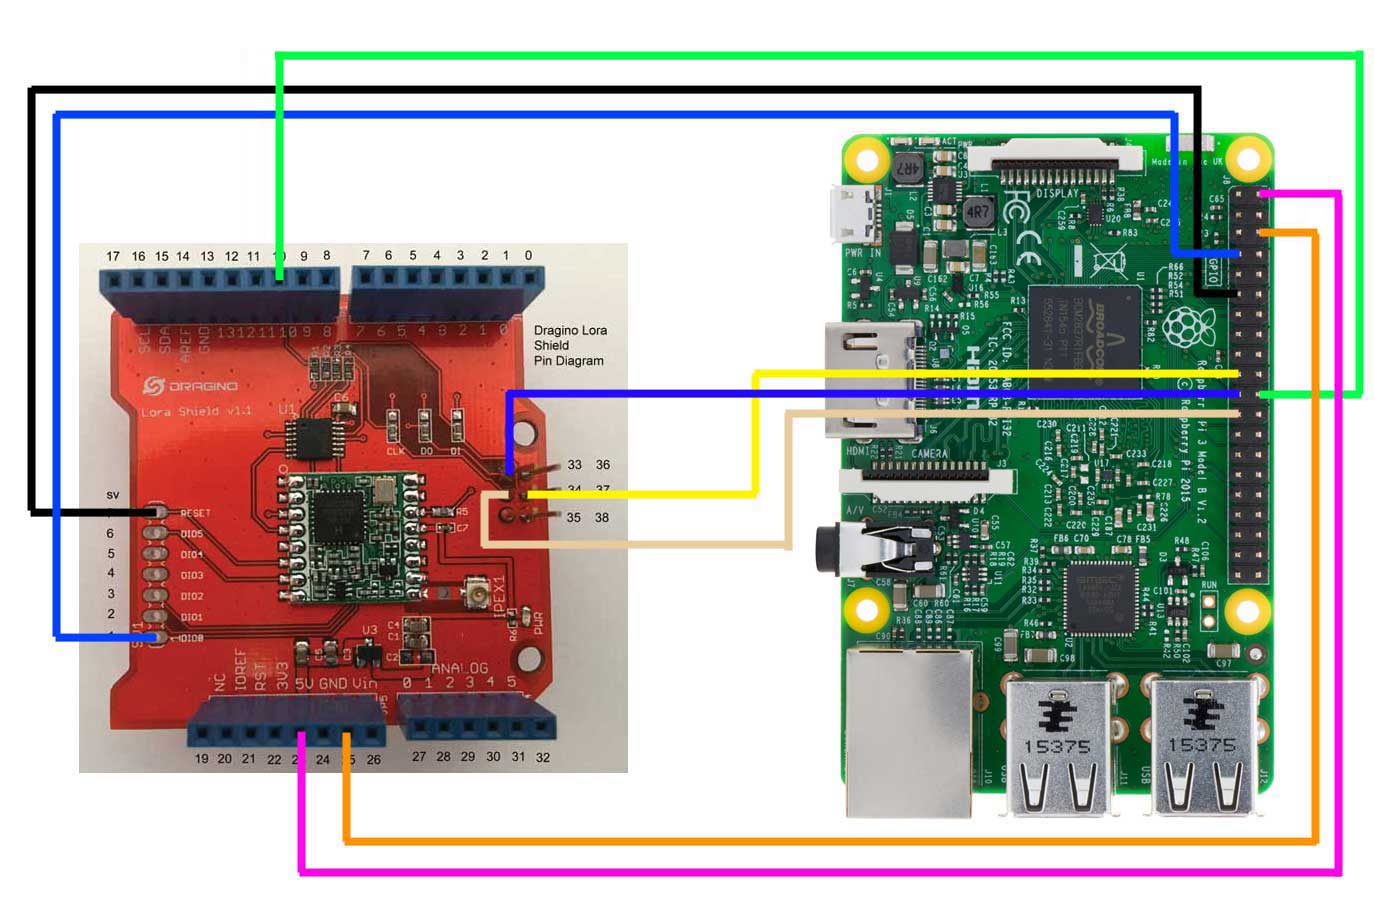
\includegraphics[scale=.2]{image6/loraras.jpg}
    \end{center}
    \caption{Kết nối giữa Lora và raspberry}
    \label{refhinh1}
    \end{figure}
\end{center}
Gateway bao gồm raspberry kết nối với Lora. Lora có nhiệm vụ kết nối với các node khác bằng sóng radio,Lora sẽ nhận tín hiệu từ các node xung quanh gửi về hoặc nó gửi giữ liệu đến các node xung quanh.Raspberry có nhiệm vụ sử lí các dữ liệu mà lora nhận được hoặc gửi đi.Raspberry kết nối với internet gửi dữ liệu lên server.\\
Nhóm đã kết nối giữa Lora và Raspberry thông qua giao thức SPI, dữ liệu có gữi và nhận giữa hai thiết bị.
\newpage
\subsection{Thực hiện kết nối giữa arduino và Lora}
\begin{center}
    \begin{figure}[htp]
    \begin{center}
     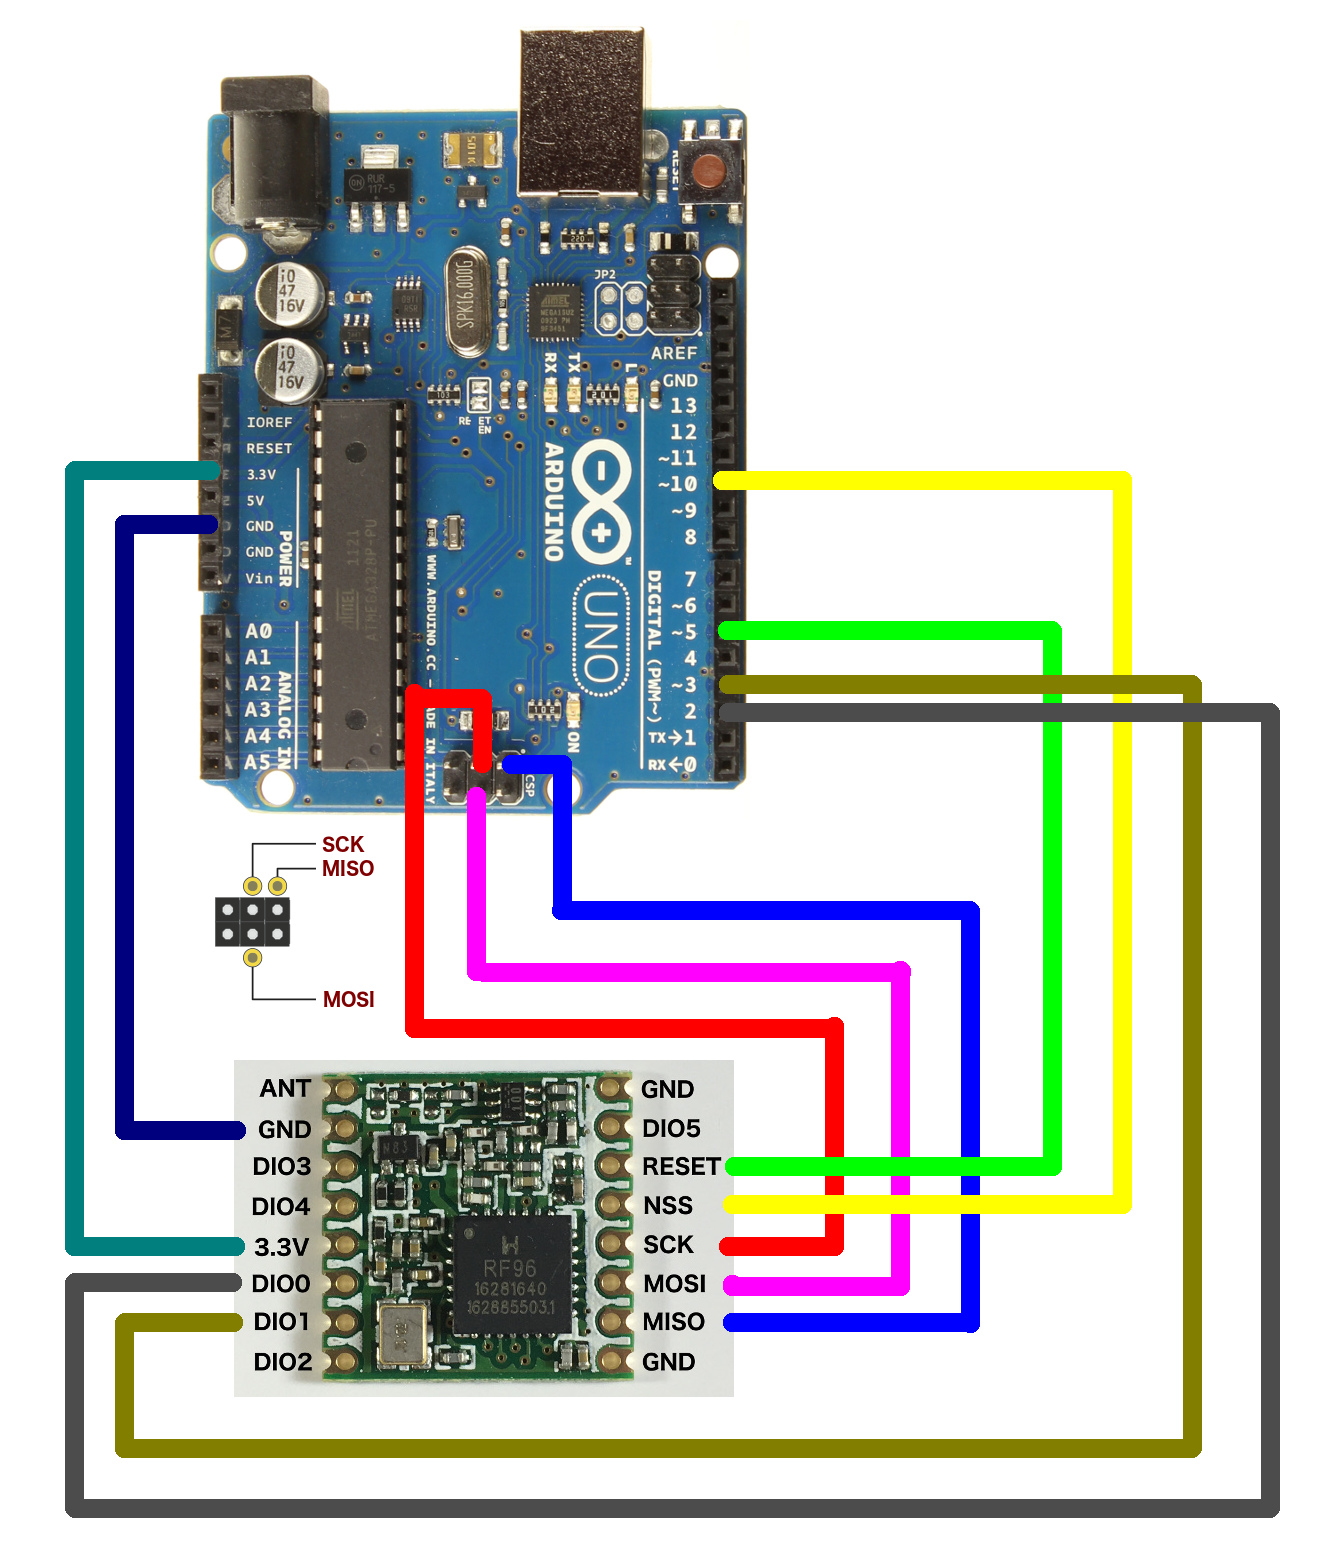
\includegraphics[scale=.2]{image6/loraar.jpg}
    \end{center}
    \caption{Kết nối giữa Lora và arduino}
    \label{refhinh1}
    \end{figure}
\end{center}
Node bao gồm arduino kết nối với Lora. Lora có nhiệm vụ kết nối với các node khác bằng sóng radio,Lora sẽ nhận tín hiệu từ các node xung quanh gửi về hoặc nó gửi giữ liệu đến các node xung quanh. Arduino có nhiệm vụ sử lí các dữ liệu mà lora nhận được hoặc gửi đi.\\
Nhóm đã kết nối giữa Lora và arduino thông qua giao thức SPI trong thư viện có sẵn của ardunio, dữ liệu có gữi và nhận giữa hai thiết bị. Hiện tại nhóm đang viết lại thư viện cho arduino và Lora
\subsection{Truyền nhận giữ liệu ở các node Lora}
Nhóm thực hiện truyền nhận dữ liệu của các node trong các trường hợp
\begin{enumerate}
    \item Thực hiện truyền nhận giữa một node server và node client.
\begin{center}
    \begin{figure}[htp]
    \begin{center}
     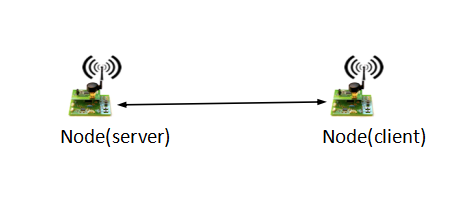
\includegraphics[scale=.8]{image6/2node.png}
    \end{center}
    \caption{Tuyền dữ liệu giữa 2 node}
    \label{refhinh1}
    \end{figure}
\end{center}
    \item Thực hiện kết nối giữa 1 node server và 2 node client
\begin{center}
    \begin{figure}[htp]
    \begin{center}
     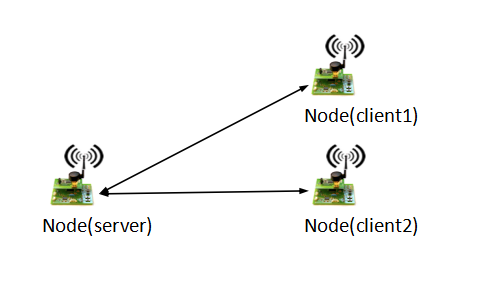
\includegraphics[scale=.8]{image6/3node.png}
    \end{center}
    \caption{Tuyền dữ liệu giữa 3 node}
    \label{refhinh1}
    \end{figure}
\end{center}
    \item Thực hiện kết nối giữa 1 node server và 3 node client
Trong trường hợp này gặp vấn đề là dữ liệu bị mất do có quá nhiều dữ liệu gửi đến và nhóm đã khác phục được
\begin{center}
    \begin{figure}[htp]
    \begin{center}
     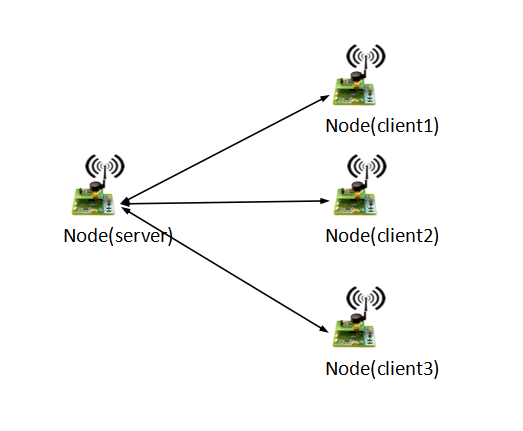
\includegraphics[scale=.8]{image6/4node.png}
    \end{center}
    \caption{Tuyền dữ liệu giữa 3 node}
    \label{refhinh1}
    \end{figure}
\end{center}
\newpage
    \item Thực hiện truyền qua các node trung gian
\begin{center}
    \begin{figure}[htp]
    \begin{center}
     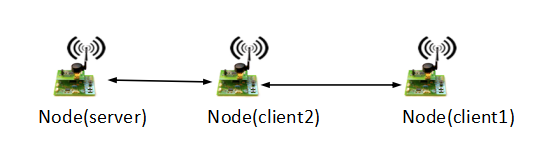
\includegraphics[scale=.8]{image6/trunggian.png}
    \end{center}
    \caption{Tuyền dữ liệu qua node trung gian}
    \label{refhinh1}
    \end{figure}
\end{center}
\end{enumerate}
\section{Hướng phát triển trong giai đoạn luận văn}
\subsection{Hiện thực server}
- Trước tiên nhóm sẽ dùng các server co sẵn để thực hiện ví dụ MQTT và Firebase\\
- Sau đó nhóm sẽ thực hiện server riêng cho mình như my sql...
\subsection{Hiện thực ứng dụng người dùng bằng ngôn ngữ hai nền tảng}
Nhóm sẽ viết phần mềm để người dùng có thể theo dõi được giữ liệu, phần có thể được phát triển ở dạng wed đối với máy tính và app đối với điện thoại.\\
Đôi với điện thoại, nhóm sẽ viết trên hai nền tảng là android và IOS.Vì đây là hai nền tảng phổ biến nhất hiện tại.\\
Dữ liệu sẽ được máy tính và điện thoại lấy từ server, cấu trúc dữ liệu bao gồm:
\begin{enumerate}
    \item Nhiệt độ
    \item Độ ẩm
    \item Thời gian
    \item Địa chỉ ID
\end{enumerate}
Dữ liệu sẽ được lưu trữ và được vẽ biểu đồ để người sử dụng có thể dễ quan sát và đưa ra nhận định.
\subsection{Thực hiện kết nối nhiều node}
Nhóm sẽ thực hiện kết nối nhiều node lora trong tự nhiên.\\
Đo xem giá trị cường độ tín hiệu nào phù hợp để kết nối.\\
Tìm thêm các thiết bị giúp sóng truyền xa hơn.\\
tìm hiểu về nguồn năng lượng mà các node sẽ sử dụng.\\
Thiết kế vỏ hộp cho các node.
%\subsection{Làm mạch}